%----------------------------------------------------------------------------------------
%	PACKAGES AND DOCUMENT CONFIGURATIONS
%----------------------------------------------------------------------------------------
% Template from Overleaf: https://www.overleaf.com/latex/templates/template-for-foundation-master-project-reports/dtzztzckwswh

\documentclass[12pt]{article}

% Adjusting margins to personal my need
\addtolength{\oddsidemargin}{-.5in}
\addtolength{\evensidemargin}{-.5in}
\addtolength{\textwidth}{1in}
\addtolength{\topmargin}{-.5in}
\addtolength{\textheight}{1in}
\setlength{\parskip}{1em}

% Graphics
\usepackage{graphicx}
\usepackage{subcaption}
\graphicspath{{figures/}}

% Math
\usepackage{amssymb}
\usepackage{amsmath} % Required for some math elements 

% Other
\usepackage{algorithmic}
\usepackage{array}
\usepackage[caption=false,font=footnotesize]{subfig}
\usepackage{lipsum}
\usepackage{hyperref}

% additional setting
\renewcommand{\abstractname}{Theme}
\usepackage[round]{natbib}
\usepackage{minted}
\usepackage{xcolor}
\definecolor{LightGray}{gray}{0.9}

%----------------------------------------------------------------------------------------
%	MAIN PART
%----------------------------------------------------------------------------------------
\begin{document}

\title{\vspace{-2cm}Logistic regression with spike-and-slab priors} 
\author{\vspace{-2cm}Wei Lu}
\date{} % Date for the report
\maketitle % Inserts the title, author and date


\begin{abstract}
%% Text of the abstract
Bayesian classification models. This project compares the logistic regression 
with normal priors and with spike-and-slab priors in terms of accuracy and uncertainty
of the posterior distributions. The frequentist's hypothesis test is employed during the comparison. The main challenges include the Rao-Blackwellization of the latent discrete
variables and the diagnostics of the binary-response model.

\end{abstract}


\section{Introduction}
Pumpkin seeds are rich in nutrients, and are widely consumed around the world. Effective Statistical models for pumpkin seeds will benefit agricultural industries and botanical studies. The dataset contains two types of pumpkins seeds (Çerçevelik, Ürgüp Sivrisi) and their morphological features. Previous studies applied machine learning methods and achieved accuracy rates about 87\% \citep{pumpkin}. In this project, the classification problem is approached with Bayesian methods. The aim is to investigate the prediction performance and the feature selection ability of the spike-and-slab prior.

\noindent\citet{selection} studied the selection of variables with hierarchical mixture models. The idea is to assign large variance to the non-zero coefficients but set small variance to zero coefficients. Consequently, the zero coefficients have "spike-like" posterior distributions and non-zero ones have widely spread distributions. \citet{sas} further improved the model with continuous priors and the rescaling method to perform variable selections on high-dimensional problems. Since the pumpkin seeds dataset has 12 features, this project employs the discrete prior model. In addition, a logistic link function is applied to address this classification problem.

\section{Analysis}

\subsection{Exploratory Data Analysis}

The prior information is important in Bayesian inference, so the exploratory analysis is conducted on the raw data. The pumpkin seed classes are nearly balanced (13:12), so the baseline accuracy is 52\% with a dummy classifier. Most distributions are unimodal and symmetric, except for "Eccentricity", "Solidity", "Extent". Hence, normal priors on the coefficients are proper choices. From the preliminary analysis, "Major\_Axis\_Length", "Eccentricity", "Roundness", "Aspect\_Ration", "Compactness" might be key features to classify the pumpkin seeds (appx. Figure \ref{fig:eda}).

\noindent Before modeling, data preprocessing is performed. The dataset is split into training data ($n=2000$) and test data ($n=500$) for the purpose of prediction. The prediction accuracy on the test data and its uncertainty are the evaluation metrics. In addition, we standardized the morphological features based on the assumptions \citep{sas}. The different value ranges caused slow-mixing issues in our model building attempts.

\subsection{Bayesian Models}
The normal-prior model is the basic Bayesian logistic regression model as the follows:
\begin{align*}
    \beta_i &\stackrel{i.i.d}\sim {\cal N}(0,10), \quad (1\leq i\leq12)\\
    \theta_j &= \text{Logistic}(X_j\underline\beta), \quad (1\leq j \leq2000) \\
     y_j &\stackrel{i.i.d}\sim \text{Bern}(\theta_j)
\end{align*}
where $X_j$ is the features of the $j^{th}$ data ($y_j$), and $\underline\beta = (\beta_1,\cdots,\beta_{12})$. The standard deviation of priors is set manually to 10.
According to \cite{selection} and \cite{sas}, the spike-and-slab hierarchical model is as the follows:
\begin{gather*}
    \sigma^2 \sim \text{InverseGamma}(\frac12,\frac12), \quad
    \tau_i^2 \stackrel{i.i.d}\sim \text{Gamma}(2,1), \quad
    p_i \stackrel{i.i.d}\sim \text{Beta}(1,1),\\ 
    \gamma_i|p_i \stackrel{i.i.d}\sim \text{Bern}(p_i), \quad
    a_i|\gamma_i,\sigma^2,\tau_i^2 = \gamma_i(v_1\sigma\tau_i) + (1-\gamma_i)\sigma\\
    \beta_i|a_i \stackrel{i.i.d}\sim {\cal N}(0,a_i), \quad
    y_j \stackrel{i.i.d}\sim \text{Bern}(\text{logistic}(X_j\underline\beta))
\end{gather*}
The $a_i$ serves as a "spike-and-slab" component, which provides a small variance for potential zero-valued $\beta_i$, and a large variance for non-zero $\beta_i$. The $v_1$ is set manually to control the "width of the slab". The zero-valued $\beta_i$'s are expected to shrink to 0, while the non-zero $\beta_i$'s are spread with large value. Note that $\gamma_i$ acts as an indicator with binary supports, Rao-Blackwellization is needed for the model implementation in Stan. Given the independency between variables, this step is simplified as the follows:
\begin{align*}
    \gamma(\beta_i,p_i,\tau_i,\sigma)&=\sum_{\gamma_i=0}^1 \gamma(\beta_i,\gamma_i,p_i,\tau_i,\sigma), \quad (1\leq i\leq 12) \\
&=f_{IG}(\sigma^2;\frac12,\frac12)f_{Gamma}(\tau_i^2;2,1)f_{Beta}(p_i;1,1)\\
&\quad \left\{ p_i\gamma_{Norm}(\beta_i;0,v_1\sigma\tau_i) + (1-p_i)\gamma_{Norm}(\beta_i;0,\sigma) \right\}
\end{align*}

\subsection{Model Diagnostics}
The MCMC methods are fast-mixing on both models. There is no obvious difference between chains in the trace plots (Figure \ref{fig:2a}, appx.\ref{fig:4a}), and the rank plots are nearly uniform (Figure \ref{fig:2b}, appx.\ref{fig:4b}). However, it is difficult to perform posterior predictive check on the binary data, since the credible set only contains 0 and 1. \citet{diag} provided some posterior check methods for discrete regressions. The simple checks for mean and standard deviation are performed. The predictions are generated with the MCMC coefficients and features of the training data. The mean and the standard deviation of the true data (brown lines) fall within the 99\% credible intervals (blue lines) of the posterior statistics (Figure \ref{fig:mixing}, appx.\ref{fig:mixing_normal}). Therefore, both models are approximately well-specified.

\begin{figure}[ht]
    \centering
    \begin{subfigure}[b]{0.45\textwidth}
        \centering
        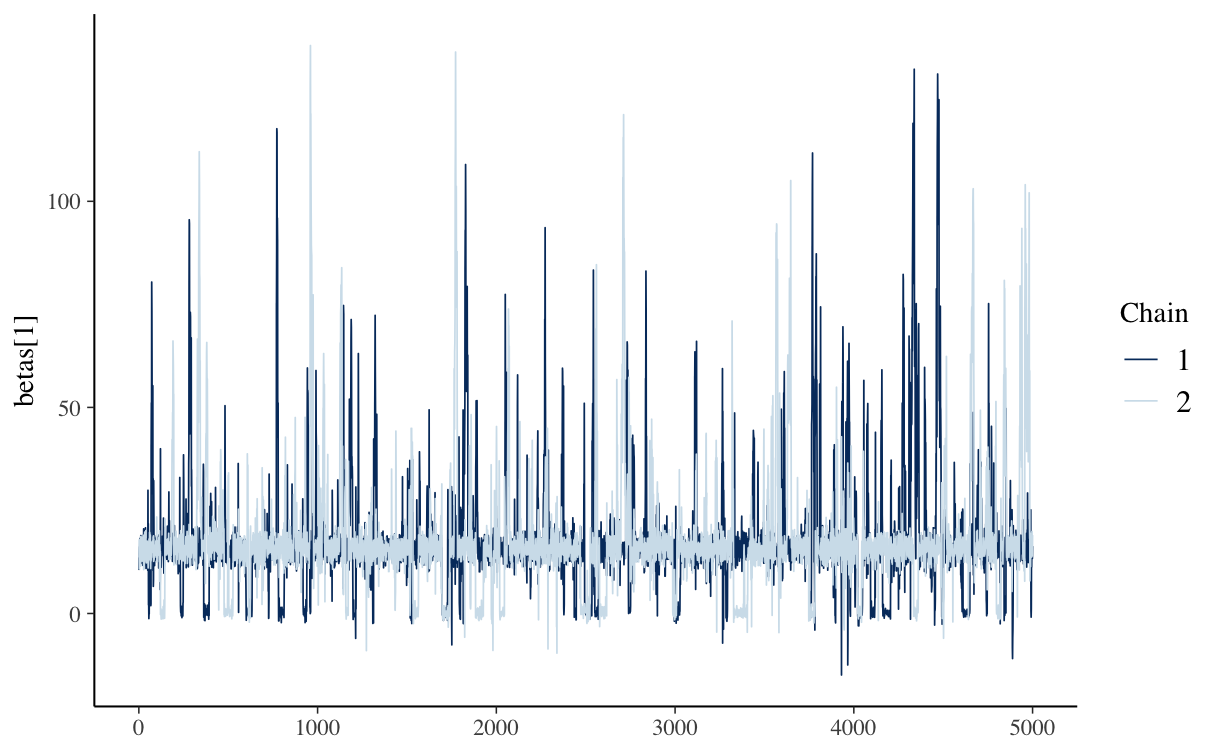
\includegraphics[width=\linewidth]{figures/trace_sas_1.png}
        \subcaption{trace plot of $\beta_1$}
        \label{fig:2a}
    \end{subfigure}
    \hfill
    \begin{subfigure}[b]{0.45\textwidth}
        \centering
        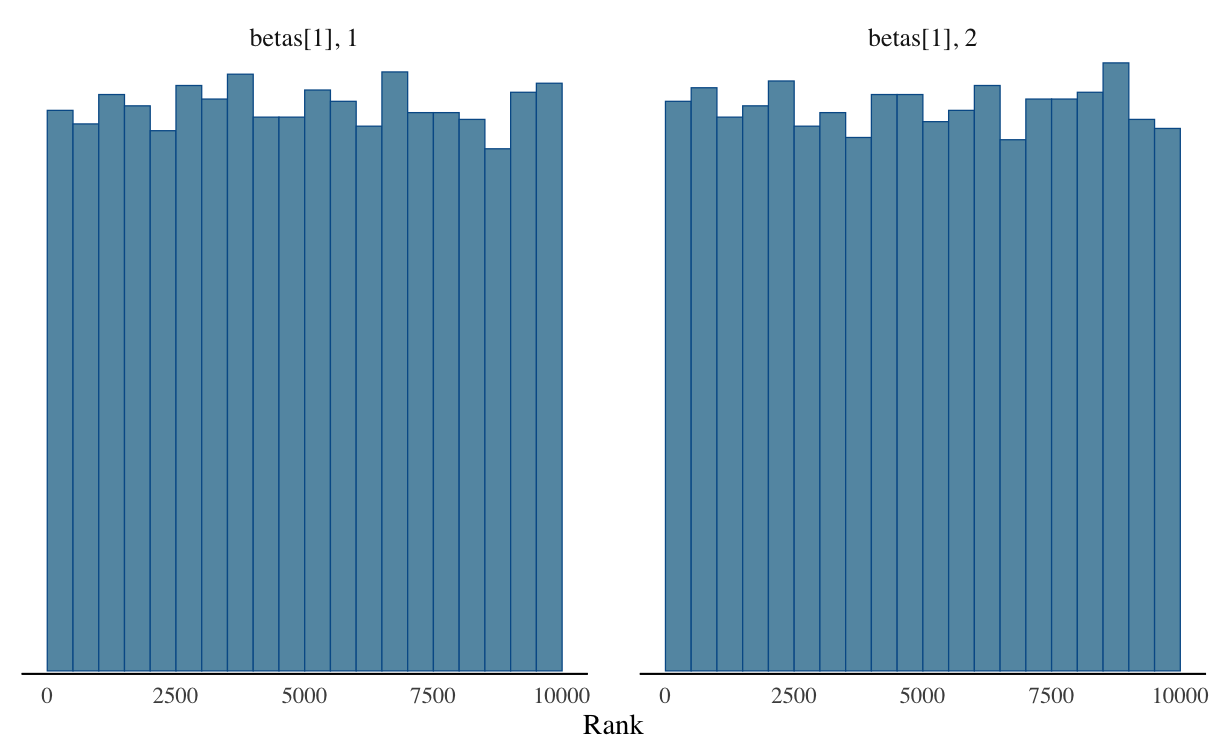
\includegraphics[width=\linewidth]{figures/rank_sas_1.png}
        \subcaption{rank plot of $\beta_1$}
        \label{fig:2b}
    \end{subfigure}

    \begin{subfigure}[b]{0.45\textwidth}
        \centering
        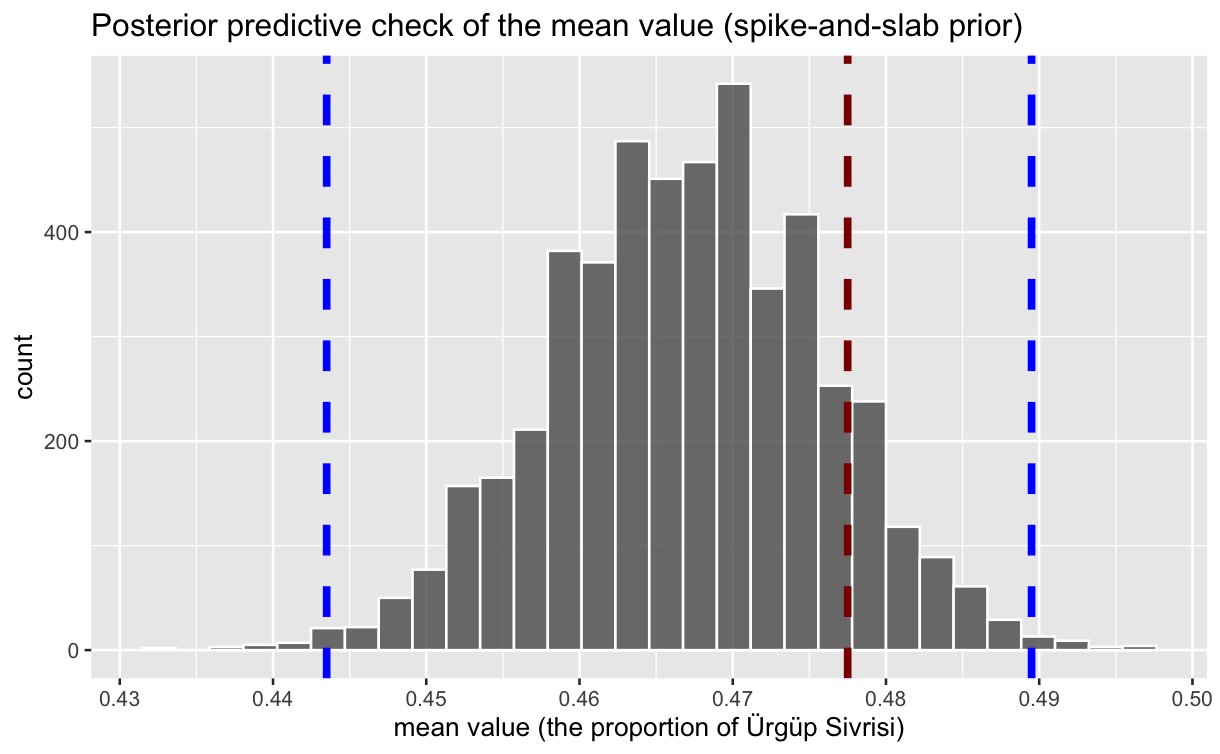
\includegraphics[width=\linewidth]{figures/ppc_sas_mean.png}
        \subcaption{predictive check for mean}
        \label{fig:2c}
    \end{subfigure}
    \hfill
    \begin{subfigure}[b]{0.45\textwidth}
        \centering
        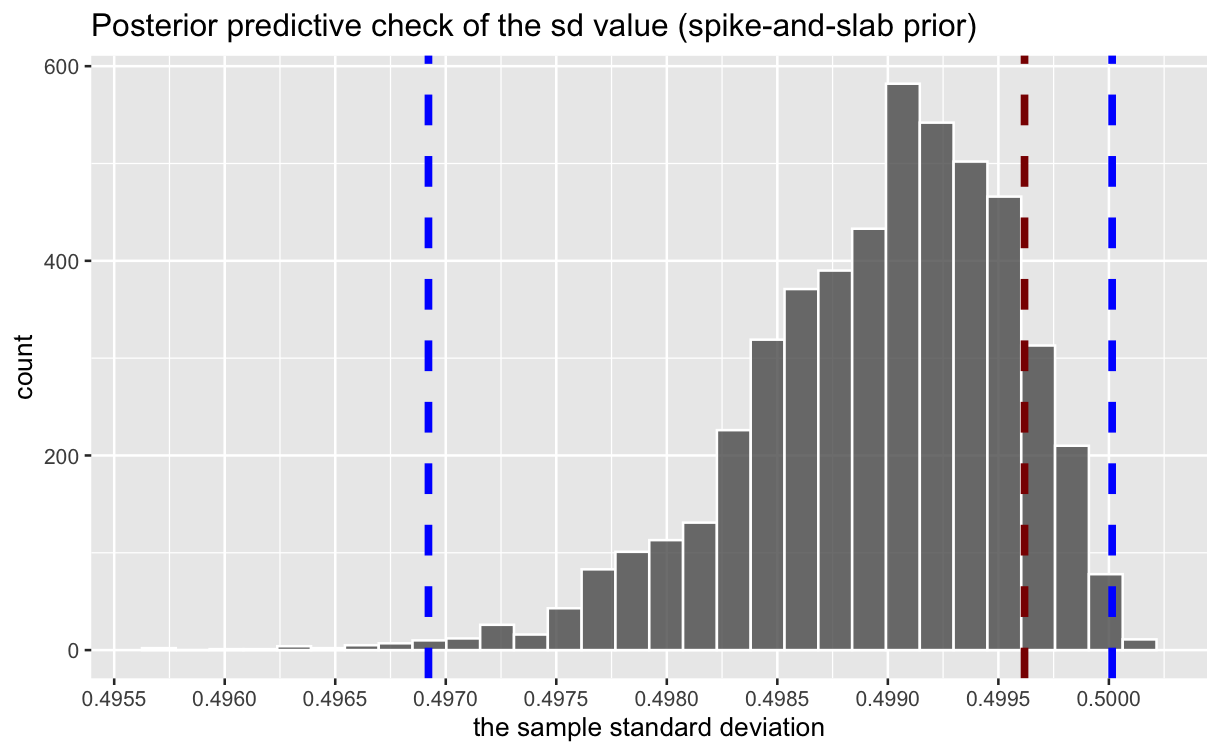
\includegraphics[width=\linewidth]{figures/ppc_sas_sd.png}
        \subcaption{predictive check for sd}
        \label{fig:2d}
        
    \end{subfigure}
    
    \caption{The diagnostics for the spike-and-slab model (partial)}
    \label{fig:mixing}
\end{figure}


\section{Results}
The posterior distributions of $\beta_2,\beta_3$ are different between two models. In particular, the distributions of the spike-and-slab model shrink to 0 with less variance, while the distributions of the normal model have larger variance and shift from 0 (Figure \ref{fig:post_23}). This discrepancy implies that "Perimeter" and "Major\_Axis\_Length" may be irrelevant morphological features to classify the pumpkin seeds. Therefore, a "reduced" model is modified from the spike-and-slab model, which excludes "Perimeter" and "Major\_Axis\_Length". Furthermore, the coefficients ($\underline\beta$) of the three models are extracted from the MCMC to simulate predictions on the test data for each iteration, resulting in accuracy distributions. With the Kolmogorov-Smirnov test, the difference of distributions is not significant between the normal and the spike-and-slab model, but the accuracy of the reduced model is significantly improved from the spike-and-slab model with less uncertainty (Table \ref{tab:ci_acc}). 

\begin{table}[ht]
\centering
\begin{tabular}{lc|c}
\hline
\textbf{Model} & \textbf{95\% CI of accuracy} & \textbf{KS p-value}\\
\hline
Normal & [0.7975 0.8280] &  0.8367 \\
Spike-and-slab & [0.7975 0.8285] & baseline \\
Reduced & [0.7980 0.8285] & 0.0017 \\
\hline
\end{tabular}
\caption{Credible intervals for accuracy and p-values}
\label{tab:ci_acc}
\end{table}




\begin{figure}[ht]
    \centering
    \begin{subfigure}[b]{0.45\textwidth}
        \centering
        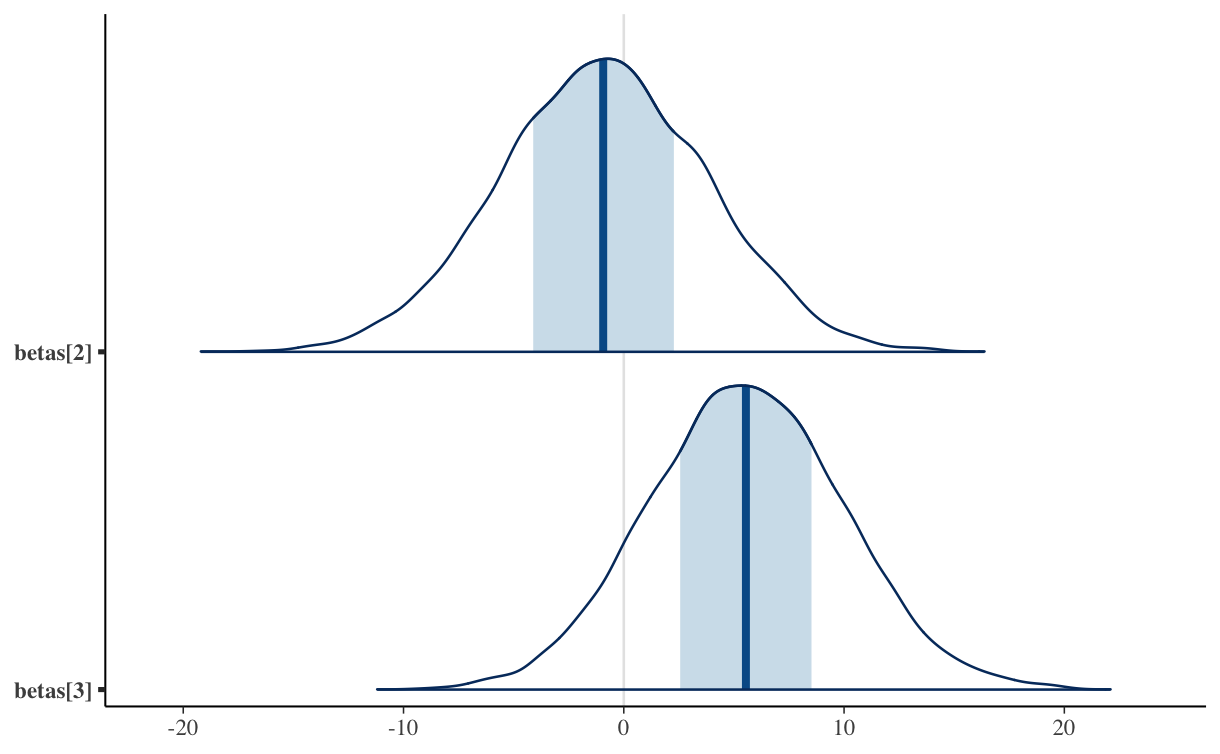
\includegraphics[width=\linewidth]{figures/post_beta_23_normal.png}
        \subcaption{normal model}
        \label{fig:3a}
    \end{subfigure}
    \hfill
    \begin{subfigure}[b]{0.45\textwidth}
        \centering
        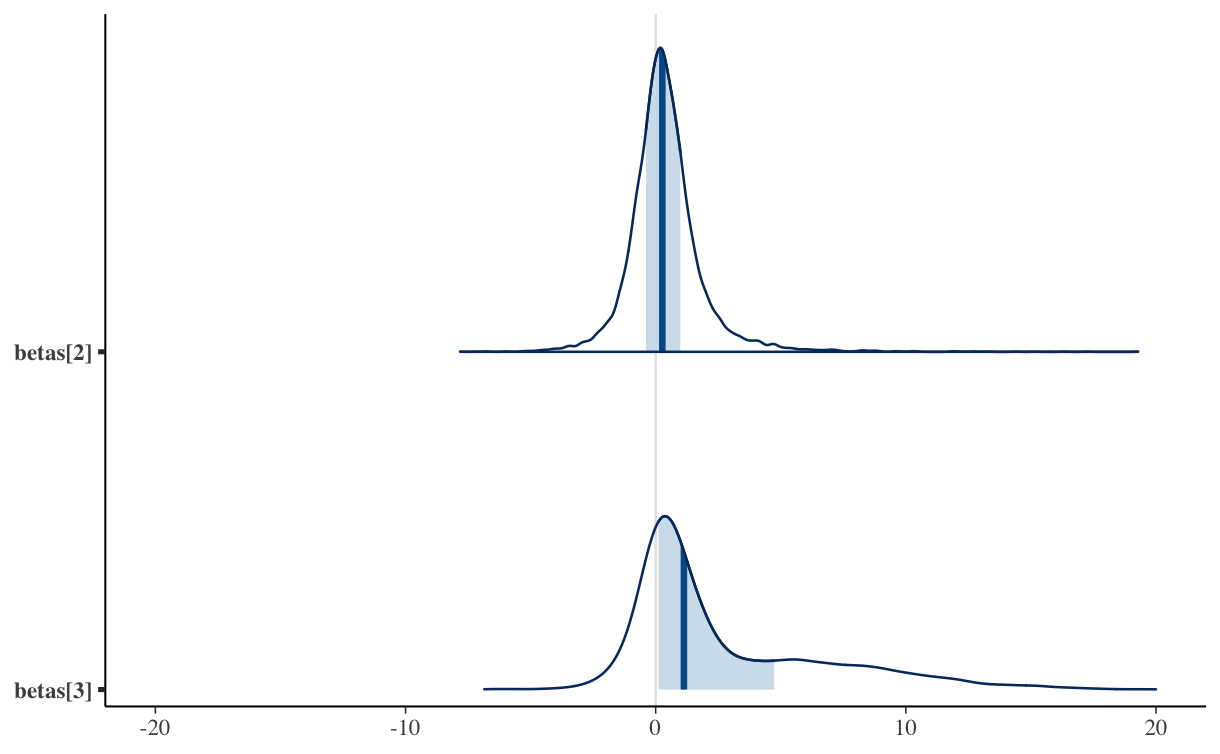
\includegraphics[width=\linewidth]{figures/post_beta23_sas.png}
        \subcaption{spike-and-slab model}
        \label{fig:3b}
    \end{subfigure}
    
    \caption{The posterior distributions of $\beta_{2,3}$}
    \label{fig:post_23}
\end{figure}

\section{Conclusion}
Both normal and spike-and-slab models have about 80\% prediction accuracy with similar uncertainty on this seed classification problem. The spike-and-slab model shows the ability to select features, resulting in a simpler reduced model with similar prediction performance, but less uncertainty. Hence, the spike-and-slab model can be further explored to study the relationships between features and give guidance to the agricultural industries.    

\noindent However, the involved features are relatively low-dimensional and non-sparse enough to show the power the the spike-and-slab prior. In addition, the spike-and-slab prior might be "washed away" during the MCMC iterations. Further studies might work on a higher dimensional sparse data with the rescaling methods \citep{sas}. 

\section{Appendix}
For more visualizations and details, see \href{https://github.com/weilu6/STAT447_Bayesian}{github.com/weilu6/STAT447\_Bayesian}.

\subsection{Stan code}
The normal model and the spike-and-slab model
\begin{minted}
[
frame=lines,
framesep=2mm,
baselinestretch=1.2,
bgcolor=LightGray,
fontsize=\footnotesize,
linenos
]
{R}
{stan output.var = "normal"}

data {
  int N; # number of train data
  int K; # number of features
  array[N] int y; # label of train
  matrix[N, K] X; # train features

}

parameters {
  vector[K] betas; # coefficients for features
}

model {
  betas ~ normal(0, 10);
  y ~ bernoulli_logit(X * betas);
}
\end{minted}

\begin{minted}
[
frame=lines,
framesep=2mm,
baselinestretch=1.2,
bgcolor=LightGray,
fontsize=\footnotesize,
linenos
]
{R}
{stan output.var = "sas"}
data {
  int N; # number of train data
  int K; # number of features
  array[N] int y; # label of train
  matrix[N, K] X; # train features
  real v_1; #control slab
}


parameters {
  real<lower=0> sigma_squared; # normal variance
  vector<lower=0>[K] tau_squared; #v ariance for each beta
  vector<lower=0.01, upper=1>[K] ps; # probability to generate 0 or 1 for indicators
  #vector[K] as; spike and slab component, no more needed since Blackwellization
  vector[K] betas; # coefficients
}

transformed parameters {
  real<lower=0> sigma = sqrt(sigma_squared); # for normal implementation, need std
  vector<lower=0>[K] tau = sqrt(tau_squared);
}

model {
  ps ~ beta(1, 1); # prior for p_i
  sigma_squared ~ inv_gamma(0.5,0.5); # prior for sigma
  tau_squared ~ gamma(2,1); # prior for tau
  #Blackwellization over Bernoulli
  for (i in 1:K) {
    target += log_sum_exp(
    log(ps[i])+gamma_lpdf(tau_squared[i]|2,1)+normal_lpdf(betas[i]|0,v_1*tau[i]*sigma),
    log(1-ps[i])+normal_lpdf(betas[i]|0,sigma));
}
  y ~ bernoulli_logit(X * betas);
}
\end{minted}


\subsection{Visualization}

\begin{figure}[ht]
    \centering
    \begin{subfigure}[b]{0.45\textwidth}
        \centering
        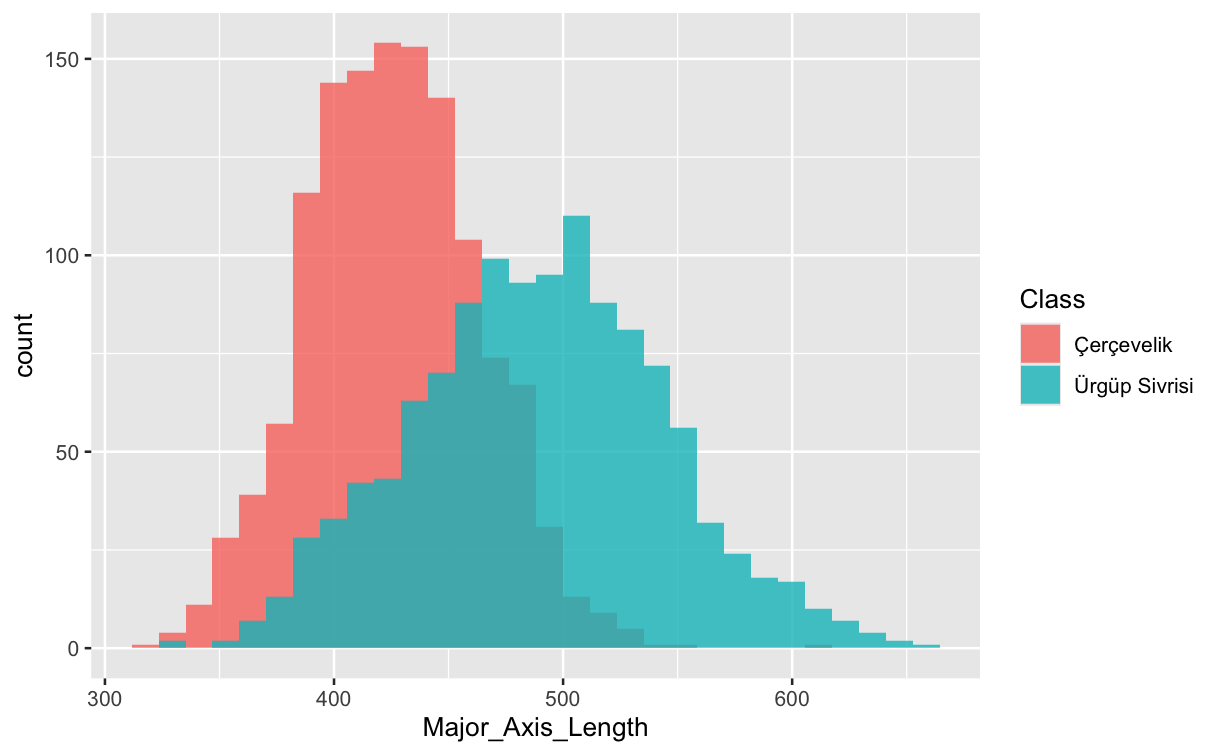
\includegraphics[width=\linewidth]{figures/EDA_1.png}
        \label{fig:1a}
    \end{subfigure}
    \hfill
    \begin{subfigure}[b]{0.45\textwidth}
        \centering
        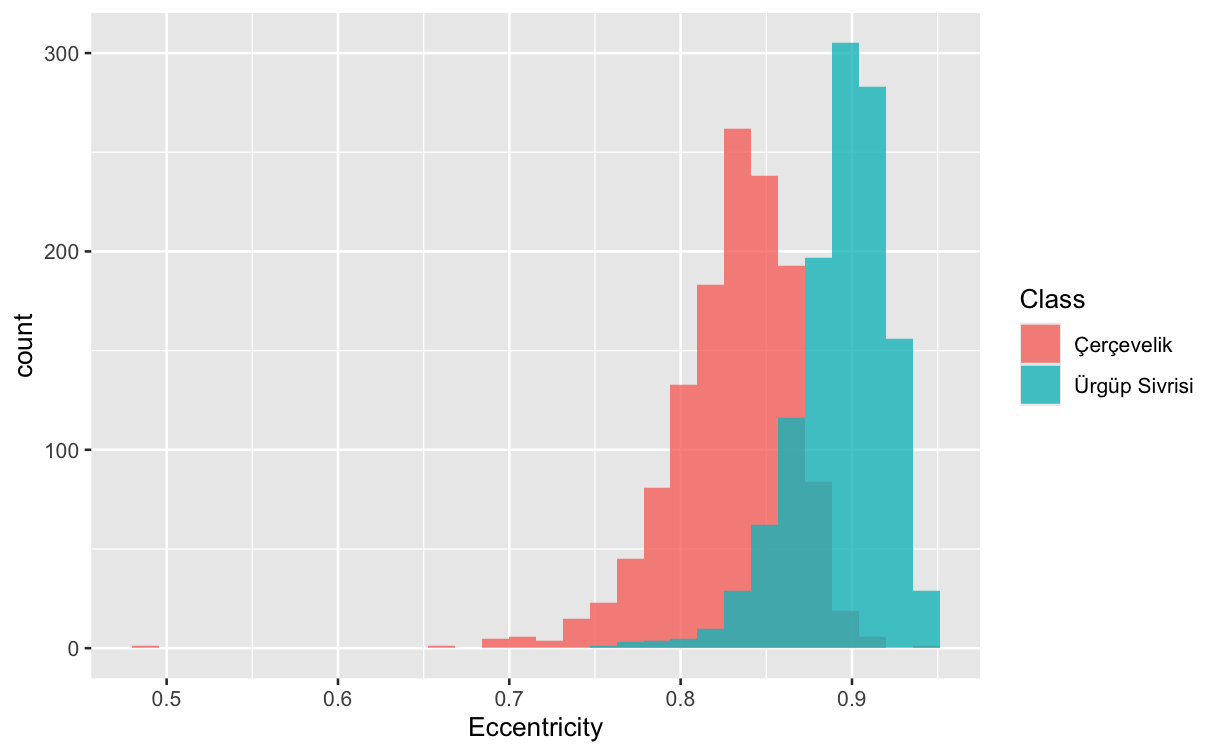
\includegraphics[width=\linewidth]{figures/EDA_2.png}
        \label{fig:1b}
    \end{subfigure}
    
    \caption{The histograms for morphological features (partial)}
    \label{fig:eda}
\end{figure}

\begin{figure}[ht]
    \centering
    \begin{subfigure}[b]{0.45\textwidth}
        \centering
        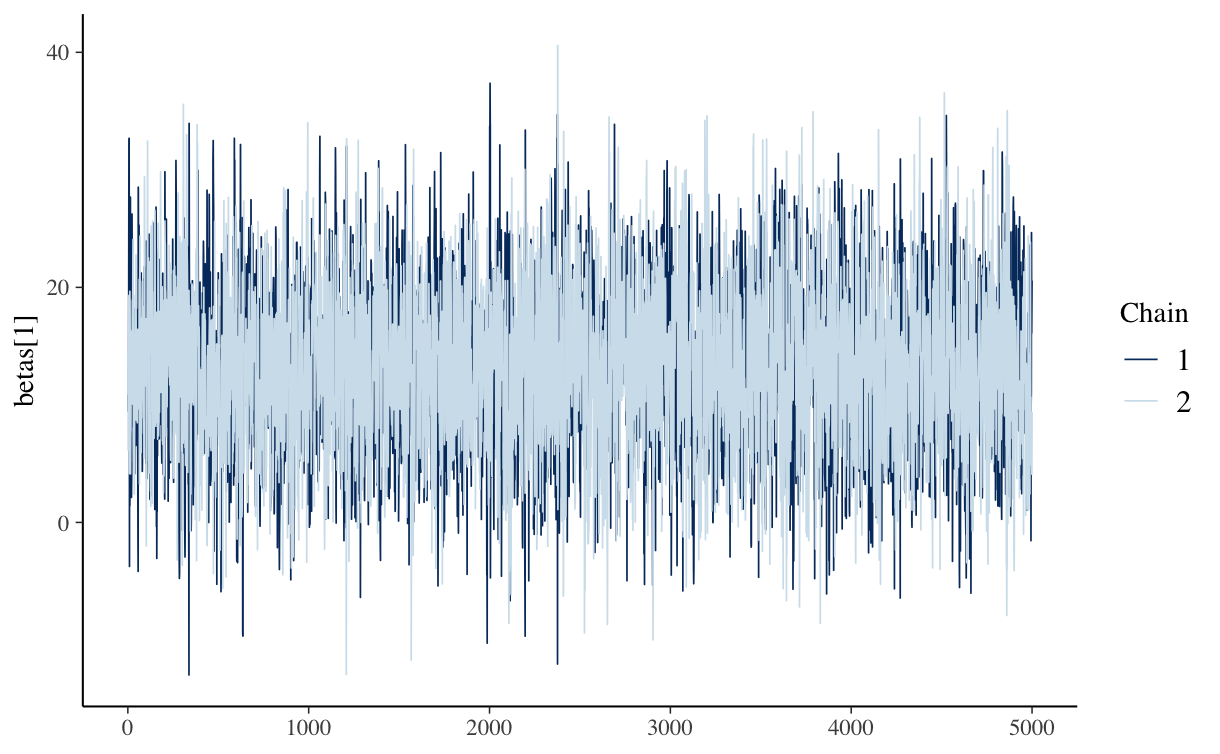
\includegraphics[width=\linewidth]{figures/trace_normal_1.png}
        \subcaption{trace plot of $\beta_1$}
        \label{fig:4a}
    \end{subfigure}
    \hfill
    \begin{subfigure}[b]{0.45\textwidth}
        \centering
        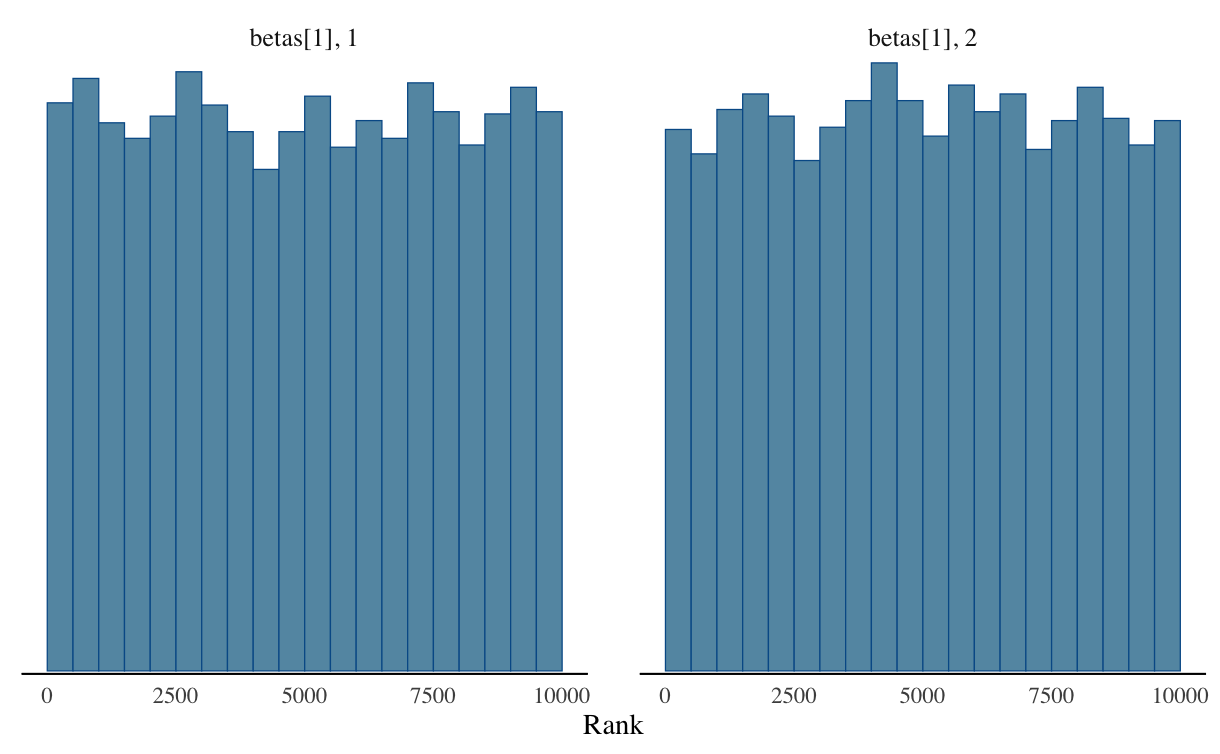
\includegraphics[width=\linewidth]{figures/rank_normal_1.png}
        \subcaption{rank plot of $\beta_1$}
        \label{fig:4b}
    \end{subfigure}

    \begin{subfigure}[b]{0.45\textwidth}
        \centering
        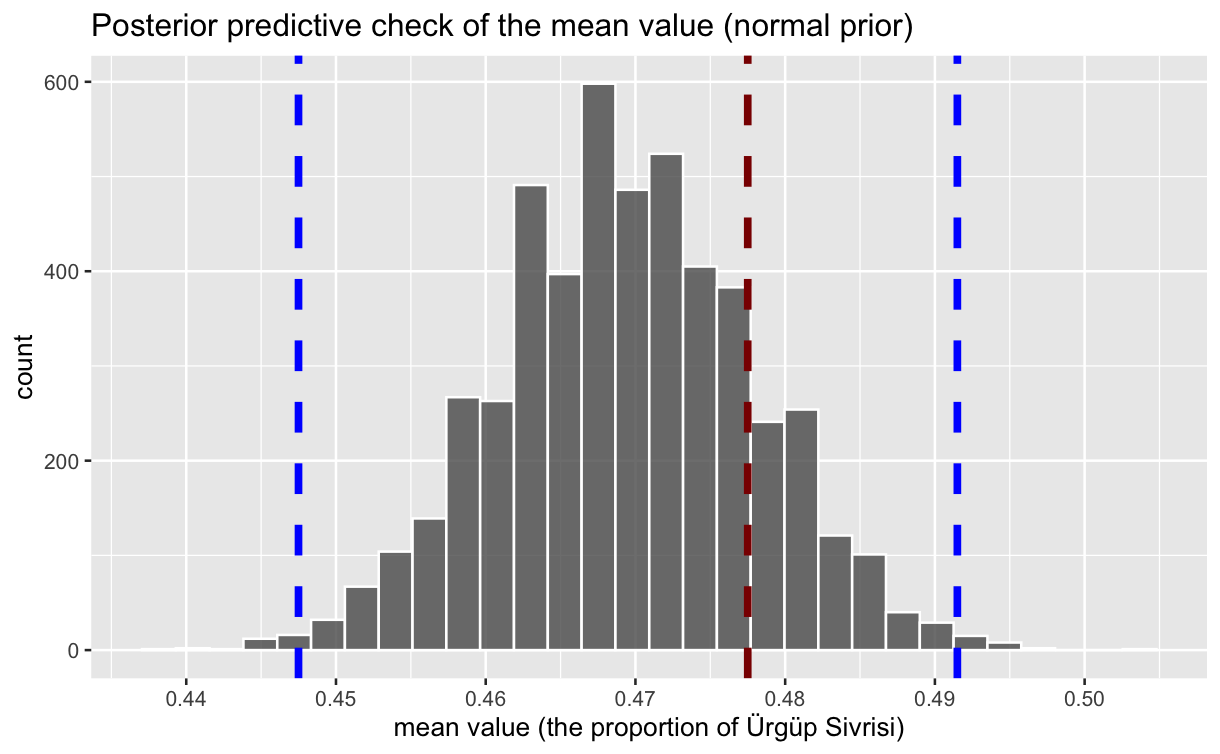
\includegraphics[width=\linewidth]{figures/ppc_normal_mean.png}
        \subcaption{predictive check for mean}
        \label{fig:4c}
    \end{subfigure}
    \hfill
    \begin{subfigure}[b]{0.45\textwidth}
        \centering
        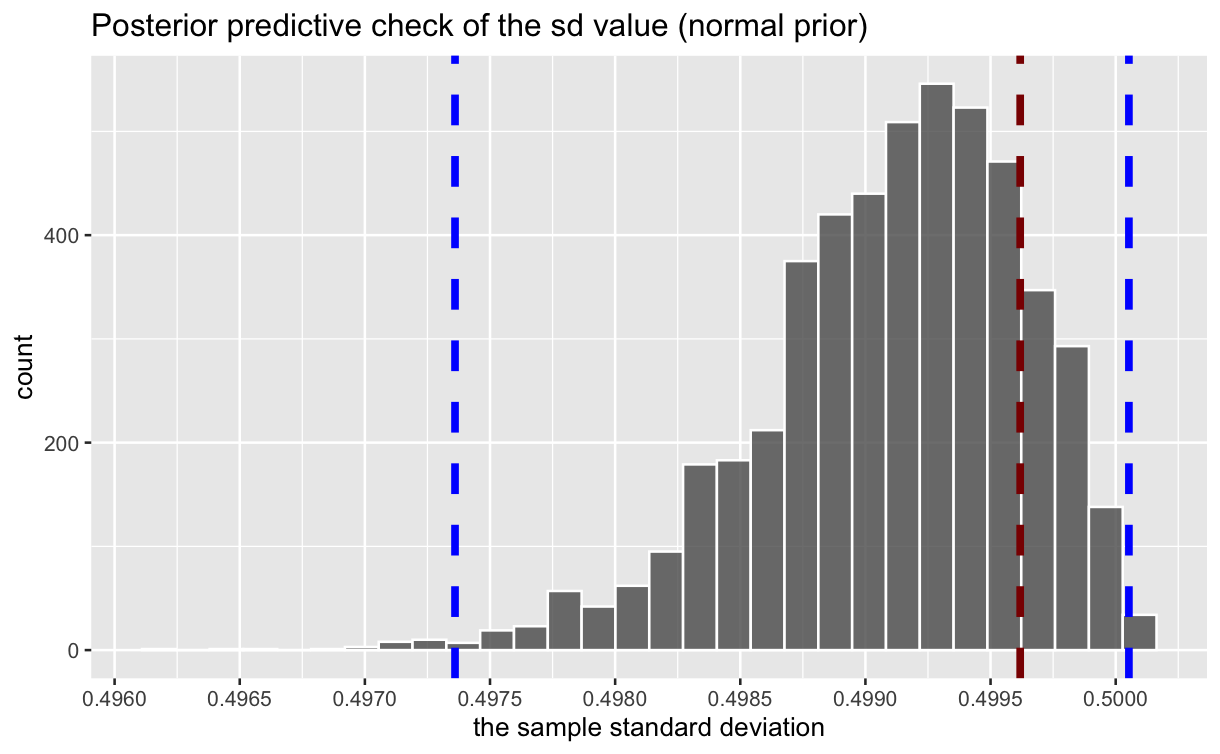
\includegraphics[width=\linewidth]{figures/ppc_normal_sd.png}
        \subcaption{predictive check for sd}
        \label{fig:4d}
        
    \end{subfigure}
    
    \caption{The diagnostics for the normal model (partial)}
    \label{fig:mixing_normal}
\end{figure}



%----------------------------------------------------------------------------------------
%	Bibliography
%----------------------------------------------------------------------------------------
\bibliography{bibliography/pumpkin_seeds}
\bibliographystyle{plainnat}

\end{document}